\documentclass[10pt, aspectratio=169]{beamer}

\usetheme[progressbar=frametitle, sectionpage=progressbar, subsectionpage=progressbar, numbering=fraction, block=fill]{metropolis}

\definecolor{mLightBrown}{HTML}{4D4D4D}
\definecolor{mMediumBrown}{HTML}{2C2C2A}
\definecolor{mDarkBrown}{HTML}{1A1A19}
\definecolor{mDarkTeal}{HTML}{0F6E56}
\definecolor{mDarkRed}{HTML}{B03A2E}
\setbeamercolor{normal text}{fg=mDarkBrown}
\setbeamercolor{alerted text}{fg=mDarkTeal}
\setbeamercolor{frametitle}{bg=mDarkBrown}
\setbeamercolor{progress bar}{fg=mDarkTeal, bg=mDarkTeal!20}
\definecolor{mPaleBg}{HTML}{F4F3EE}
\setbeamercolor{block title}{bg=mDarkBrown!10, fg=mDarkBrown}
\setbeamercolor{block body}{bg=mPaleBg, fg=mDarkBrown}
\newcommand{\hl}[1]{\textcolor{mDarkTeal}{#1}}

\usepackage{amsmath, amssymb, amsthm, mathtools}
\usepackage{cancel}\usepackage{bm}\usepackage{booktabs}\usepackage{array}
\usepackage{xcolor}\usepackage{colortbl}\usepackage{multirow}\usepackage{tikz}
\usetikzlibrary{positioning,arrows.meta,calc,fit,shapes.geometric,decorations.pathmorphing}

\newcommand{\paper}[1]{\textcolor{mLightBrown}{\small\textit{(#1)}}}

\newcommand{\qcur}{0}
\newcommand{\qnode}[4]{%
\ifnum#4=\qcur
 \node[draw=mDarkTeal, fill=mDarkTeal!12, thick, rounded corners=1pt, minimum width=3.0cm, minimum height=0.52cm, font=\tiny\bfseries, text=mDarkBrown] (#2) at (#1,0) {#3};%
\else
 \node[draw=mLightBrown!45, rounded corners=1pt, minimum width=3.0cm, minimum height=0.52cm, font=\tiny, text=mLightBrown] (#2) at (#1,0) {#3};%
\fi}
\newcommand{\qstrip}[1]{\renewcommand{\qcur}{#1}%
\begin{center}
\begin{tikzpicture}
\qnode{0}{q1}{Q1 Offline?}{1}
\qnode{3.7}{q2}{Q2 Why fail?}{2}
\qnode{7.4}{q3}{Q3 Conservative?}{3}
\qnode{11.1}{q4}{Q4 Robust?}{4}
\draw[-{Stealth}, mLightBrown!60] (q1.east) -- (q2.west);
\draw[-{Stealth}, mLightBrown!60] (q2.east) -- (q3.west);
\draw[-{Stealth}, mLightBrown!60] (q3.east) -- (q4.west);
\end{tikzpicture}\end{center}}

\title{Data-Driven Design Optimization --- Surrogate-Based}
\subtitle{A surrogate you optimize against will be exploited where it is wrong}
\author{Jinkyoo Park}
\institute{KAIST}
\date{\textit{Lecture 5 --- Offline optimization, part 1 of 2: approximate the function, then search}}

\begin{document}

\maketitle

%==========================================================
\section{The handoff --- optimization with no oracle}
%==========================================================

\begin{frame}{Where we are --- the query is taken away}
\vspace{2pt}
Lecture 4 could \alert{query} the expensive function $f$ whenever it wished. Often you cannot: the data is already collected and \alert{fixed} --- a database of proteins and their activity, of alloys and their strength, of designs and their performance. No new experiments.
\medskip

\pause
The problem statement is shared with the next lecture, and it is exactly Lecture 1's goal under a harsh new constraint:
\[
\text{find}\quad x^* = \arg\max_x f(x) \qquad \text{with \alert{only} a fixed dataset } D = \{(x_i, f(x_i))\}_{i=1}^N.
\]
\medskip

\pause
This is \alert{offline model-based optimization}. Two routes exist; this lecture takes the first:
\begin{enumerate}\setlength\itemsep{1pt}
\item \textbf{Surrogate-based} (today): approximate $f$ from $D$, then optimize \emph{over the surrogate}.
\item \textbf{Generative-based} (Lecture 6): learn the inverse map and \emph{sample} good designs directly.
\end{enumerate}
\end{frame}

\begin{frame}{The thesis --- the surrogate's blind spots are where you'll be sent}
The fixed point of this lecture, in one line:
\begin{center}\large
\alert{An optimizer turned loose on a learned surrogate will seek out exactly the inputs where the surrogate is wrongly optimistic.}
\end{center}
\medskip

\pause
It sounds like Lecture 4 again --- fit a model of $f$, optimize it --- but offline the danger is far sharper. In BO we could \emph{check} a promising point by querying it. Offline we cannot: a design the surrogate loves but that is actually terrible will simply be \alert{returned as the answer}.
\medskip

\pause
So the whole lecture is about one failure and its cure: the surrogate \alert{overestimates} far from data, the optimizer \alert{exploits} that overestimation, and the fix is to make the surrogate deliberately \alert{conservative} where it has no evidence.
\end{frame}

\begin{frame}{The roadmap --- four questions}
\qstrip{0}
\medskip
\begin{itemize}\setlength\itemsep{3pt}
\item \textbf{Q1 --- What changes when optimization goes offline?} No oracle to check a candidate.
\item \textbf{Q2 --- Why does the naive ``fit and ascend'' fail?} \alert{Overestimation} on the narrow valid manifold.
\item \textbf{Q3 --- How do we fix it?} \alert{Conservative objective models} --- penalize the surrogate where the optimizer attacks.
\item \textbf{Q4 --- What else helps?} Uncertainty (NEMO) and local smoothness (RoMA).
\end{itemize}
\end{frame}

%==========================================================
\section{Act 1 --- the naive approach}
%==========================================================

\begin{frame}{The obvious method --- fit a proxy, then climb it}
\qstrip{1}
\medskip
The straightforward recipe, supervised learning then optimization:
\[
\textbf{Step 1.}\quad \theta^* = \arg\min_\theta \frac1N\sum_{i=1}^N \big(f_\theta(x_i) - f(x_i)\big)^2,
\qquad
\textbf{Step 2.}\quad x^* = \arg\max_x f_{\theta^*}(x).
\]
\medskip
Fit a neural network $f_\theta$ to the data (a \alert{surrogate} / proxy), then do gradient ascent on it to find the best input.
\medskip

\pause
This is just Lecture 4's loop with the active query removed --- learn the function, optimize the function. On paper it should work. In high dimensions, it fails badly --- and understanding \emph{why} is the lecture.
\end{frame}

%==========================================================
\section{Act 2 --- why it fails}
%==========================================================

\begin{frame}{The failure --- the optimizer is an adversary}
\qstrip{2}
\medskip
Two facts collide:
\begin{itemize}\setlength\itemsep{2pt}
\item \textbf{The valid manifold is narrow.} In protein/image/design spaces, only a thin sliver of the high-dimensional input space is meaningful; the rest is garbage.
\item \textbf{Neural nets overestimate off-manifold.} A network trained only on $D$ is unconstrained where it has no data --- and tends to predict \alert{wildly high} values there (the surface is non-smooth).
\end{itemize}
\medskip

\pause
Gradient ascent then does the worst possible thing: it climbs toward those \alert{out-of-distribution} peaks --- regions where $f_\theta$ is high precisely \emph{because} it is wrong.
\medskip
\begin{center}\large
The optimizer behaves like an \alert{adversarial attack} on the surrogate.
\end{center}
\medskip

\pause
(Recall: a tiny crafted perturbation flips a classifier's ``panda'' to ``gibbon'' at 99\% confidence. Gradient ascent on $f_\theta$ is the same mechanism --- it manufactures inputs the model rates highly but that are meaningless.)
\end{frame}

\begin{frame}{The picture --- climbing into a hallucinated peak}
\begin{center}
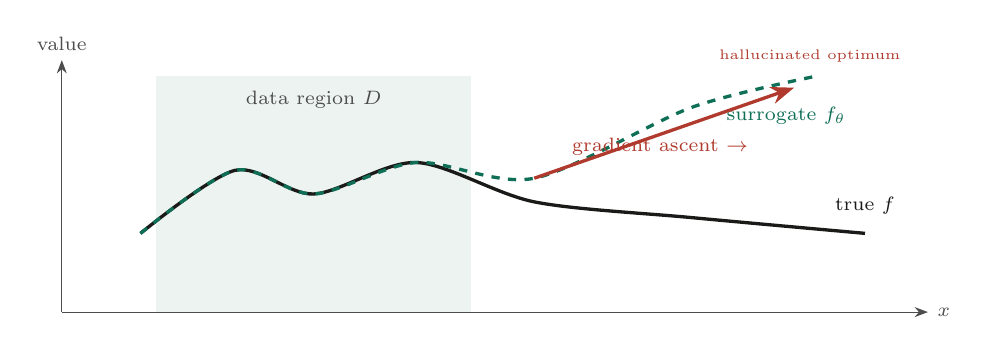
\begin{tikzpicture}[font=\scriptsize]
% true function (dark) and surrogate (teal) diverging off-data
\draw[-{Stealth}, mLightBrown] (0,0) -- (11,0) node[right]{$x$};
\draw[-{Stealth}, mLightBrown] (0,0) -- (0,3.2) node[above]{value};
% data region shaded
\fill[mDarkTeal!8] (1.2,0) rectangle (5.2,3.0);
\node[mLightBrown] at (3.2,2.7) {data region $D$};
% true f
\draw[mDarkBrown, very thick] plot[smooth] coordinates {(1.0,1.0)(2.2,1.8)(3.2,1.5)(4.5,1.9)(6.0,1.4)(8.0,1.2)(10.2,1.0)};
\node[mDarkBrown] at (10.2,1.35) {true $f$};
% surrogate: matches in data, shoots up outside
\draw[mDarkTeal, very thick, dashed] plot[smooth] coordinates {(1.0,1.0)(2.2,1.8)(3.2,1.5)(4.5,1.9)(6.0,1.7)(8.0,2.6)(9.6,3.0)};
\node[mDarkTeal] at (9.2,2.5) {surrogate $f_\theta$};
% optimizer arrow climbing OOD
\draw[-{Stealth}, mDarkRed, very thick] (6.0,1.7) -- (9.3,2.85);
\node[mDarkRed] at (7.6,2.1) {gradient ascent $\to$};
\node[mDarkRed, font=\tiny] at (9.5,3.25) {hallucinated optimum};
\end{tikzpicture}
\end{center}
\medskip

\pause
Inside the data region, surrogate and truth agree. Outside, the surrogate drifts upward with no penalty --- and that is exactly where the optimizer goes. The returned $x^*$ is a confident fiction.
\medskip
\begin{center}\large
The cure is not a better optimizer --- it is a \alert{more honest surrogate}.
\end{center}
\end{frame}

%==========================================================
\section{Act 3 --- conservative objective models}
%==========================================================

\begin{frame}{COMs --- train the surrogate to distrust its own optimizer}
\qstrip{3}
\medskip
\textbf{Conservative Objective Models} \paper{Trabucco et al., 2021}: learn a surrogate that \emph{does not overestimate} the very inputs an optimizer would chase. The trick is to generate those inputs during training.
\medskip

\pause
\textbf{Find the adversaries.} Roll out gradient ascent \emph{on the current surrogate}, starting from data, to produce the distribution $\mu(x)$ of points it would be tempted by:
\[
\mu(x) = \Big\{\textstyle\sum_t \delta_{x_t}: \ x_{t+1} = x_t + \eta\,\nabla_{x_t} f_\theta(x_t),\ x_0 \sim D\Big\}.
\]
\medskip

\pause
\textbf{Push them down, hold the data up.} Train with a conservative regularizer:
\[
L(\theta) = \underbrace{\tfrac12 \mathbb{E}_{(x,y)\sim D}\big[(f_\theta(x)-y)^2\big]}_{\text{fit the data}} \;+\; \alpha\Big(\underbrace{\mathbb{E}_{x\sim\mu(x)}[f_\theta(x)]}_{\text{\hl{lower OOD peaks}}} - \underbrace{\mathbb{E}_{x\sim D}[f_\theta(x)]}_{\text{don't crush data}}\Big).
\]
\end{frame}

\begin{frame}{Why COMs works --- a learned lower bound}
\begin{center}\large
The two penalty terms together pull the surrogate \alert{down where the optimizer attacks}, while \alert{holding it up on real data}.
\end{center}
\medskip
\begin{itemize}\setlength\itemsep{2pt}
\item without the second term, the surrogate would collapse everywhere (underestimation);
\item with both, $f_\theta$ becomes a \alert{conservative lower bound} on the true function off-distribution, accurate on-distribution;
\item now gradient ascent has nowhere fake to climb --- the hallucinated peaks have been flattened.
\end{itemize}
\medskip

\pause
\begin{center}
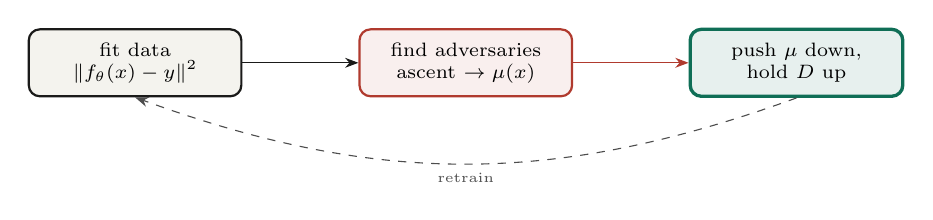
\begin{tikzpicture}[font=\scriptsize, node distance=4pt]
\node[draw=mDarkBrown, thick, fill=mPaleBg, rounded corners, minimum width=2.7cm, minimum height=0.85cm, align=center] (a) at (0,0) {fit data\\ \scriptsize $\|f_\theta(x)-y\|^2$};
\node[draw=mDarkRed, thick, fill=mDarkRed!8, rounded corners, minimum width=2.7cm, minimum height=0.85cm, align=center] (b) at (4.2,0) {find adversaries\\ \scriptsize ascent $\to \mu(x)$};
\node[draw=mDarkTeal, very thick, fill=mDarkTeal!10, rounded corners, minimum width=2.7cm, minimum height=0.85cm, align=center] (c) at (8.4,0) {push $\mu$ down,\\ hold $D$ up};
\draw[-{Stealth}, mDarkBrown] (a)--(b); \draw[-{Stealth}, mDarkRed] (b)--(c);
\draw[-{Stealth}, mLightBrown, dashed] (c.south) to[bend left=20] node[below,font=\tiny]{retrain} (a.south);
\end{tikzpicture}
\end{center}
\medskip
\pause
The structure is simple: it is ordinary supervised regression plus one adversarial term --- standard optimizers still apply. Conservatism is the whole idea.
\end{frame}

%==========================================================
\section{Act 4 --- other ways to be robust}
%==========================================================

\begin{frame}{NEMO and RoMA --- uncertainty and smoothness}
\qstrip{4}
\medskip
COMs is one answer to overestimation; two others attack the same disease differently.
\medskip
\begin{itemize}\setlength\itemsep{4pt}
\item \textbf{NEMO} --- handle overestimation as \alert{uncertainty}. Use a Normalized Maximum Likelihood estimator (with a tractable approximation) so the surrogate \emph{knows what it doesn't know}, and the optimizer is steered away from high-uncertainty regions. \paper{NML-based}
\item \textbf{RoMA} --- enforce \alert{local smoothness} at the points the optimizer visits. As gradient ascent proceeds, re-adapt the model to be smooth at the current candidate:
\[
\theta_t = \arg\min_{\tilde\theta\in B(\theta)} \big\|\nabla_x f(x_t;\tilde\theta)\big\|^2 + \alpha\big(f(x_t;\tilde\theta) - f(x_t;\theta_{t-1})\big)^2,
\]
so updates don't run off into non-smooth, hallucinated regions.
\end{itemize}
\medskip

\pause
\begin{center}\large
All three say the same thing: \alert{respect uncertainty off-distribution}, or the optimizer will weaponize it.
\end{center}
This is Lecture 4's lesson --- uncertainty matters --- made non-negotiable, because here there is no query to correct a mistake.
\end{frame}

%==========================================================
\section{Closing}
%==========================================================

\begin{frame}{Where we are --- forward model, then search}
\vspace{2pt}
\begin{center}\footnotesize\renewcommand{\arraystretch}{1.45}
\begin{tabular}{l|c|c}
 & \textbf{the model} & \textbf{the decision} \\
\hline
\textbf{Surrogate (Lec.\ 5)} & \cellcolor{mDarkTeal!15}forward $f_\theta(x)\approx f$ & \cellcolor{mDarkTeal!15}optimize / search over $f_\theta$ \\
\textbf{Generative (Lec.\ 6)} & inverse $p(x\mid y)$ & sample good designs \\
\end{tabular}
\end{center}
\medskip

\pause
We solved offline design one way: build a \emph{forward} surrogate of $f$, then \emph{search} it --- carefully, conservatively, so the search cannot exploit our ignorance.
\medskip

\pause
But there is a completely different route. Instead of approximating $f$ and \emph{searching}, why not learn to \alert{generate} good designs directly --- the inverse map from ``I want a high value'' to ``here is an input that gives it''?
\begin{center}\large
That is Lecture 6: don't search the design --- \alert{produce} it.
\end{center}
\end{frame}

\begin{frame}{Closing --- the one sentence}
\vfill
\begin{center}\large
Offline, you cannot test a candidate --- so a surrogate's optimism becomes the optimizer's trap.\\[8pt]
The cure is conservatism:\\[4pt]
teach the model to doubt itself exactly where it will be attacked,\\[4pt]
and gradient ascent has nowhere false left to climb.
\end{center}
\vfill
\pause
\footnotesize
Hold the shape of this lecture: a \emph{forward} model of the objective, \emph{searched} for an optimum. Lecture 6 inverts every word of that --- an \emph{inverse} model, \emph{sampled} for a design --- the same duality that, in Part IV, separates value-based RL (search a value) from policy-based RL (produce an action).
\end{frame}

\begin{frame}[standout]
Questions?
\end{frame}

%==========================================================
\appendix
%==========================================================

\begin{frame}{Backup 1 --- offline MBO vs.\ Bayesian optimization}
\footnotesize
The same goal, $\arg\max_x f(x)$, under different access --- and the difference dictates the method.
\medskip
\begin{center}\scriptsize\renewcommand{\arraystretch}{1.4}
\begin{tabular}{l|l|l}
 & \textbf{Bayesian optimization (Lec.\ 4)} & \textbf{Offline MBO (Lec.\ 5)} \\
\hline
data & \emph{active} --- query $f$ each round & \emph{fixed} --- a static dataset $D$ \\
mistakes & corrected by the next query & \alert{uncorrectable} --- returned as the answer \\
uncertainty & drives \emph{where to sample} & drives \emph{where not to trust} \\
core risk & slow convergence & overestimation $\to$ invalid design \\
\end{tabular}
\end{center}
\medskip
In BO, uncertainty is an \emph{opportunity} (explore there). Offline, uncertainty is a \emph{hazard} (the optimizer will exploit it and you cannot check). Same Gaussian-process-era intuition, opposite operational consequence --- which is why the offline methods are built around \emph{conservatism} rather than \emph{exploration}.
\end{frame}

\begin{frame}{Backup 2 --- the COMs objective, term by term}
\footnotesize
\[
L(\theta) = \underbrace{\tfrac12 \mathbb{E}_{(x,y)\sim D}\big[(f_\theta(x)-y)^2\big]}_{\text{(i) supervised fit}}
\;+\; \alpha\,\underbrace{\mathbb{E}_{x\sim\mu(x)}[f_\theta(x)]}_{\text{(ii) push adversaries down}}
\;-\; \alpha\,\underbrace{\mathbb{E}_{x\sim D}[f_\theta(x)]}_{\text{(iii) hold data up}}.
\]
\begin{itemize}\setlength\itemsep{1pt}
\item \textbf{(i)} ordinary regression --- be accurate on the data we have;
\item \textbf{(ii)} the conservative term --- minimize predicted value on the adversarial distribution $\mu(x)$ (the points gradient ascent on $f_\theta$ produces). \emph{Prevents overestimation of out-of-distribution inputs};
\item \textbf{(iii)} the counter-term --- without it, (ii) would drag the whole surface down, including real data. Maximizing value on $D$ \emph{prevents underestimation of in-distribution inputs}.
\end{itemize}
\medskip
\textbf{Guarantee (informal).} Under regularity assumptions, the trained $f_\theta$ \emph{lower-bounds} the true objective off-distribution --- so the optimum of $f_\theta$ cannot be an over-optimistic hallucination. The hyperparameter $\alpha$ tunes how conservative.
\end{frame}

\begin{frame}{Backup 3 --- generating the adversarial distribution}
\footnotesize
The adversarial distribution $\mu(x)$ is built by simulating the very attack we fear.
\[
\mu(x) = \Big\{\textstyle\sum_{t} \delta_{x_t} : \quad x_0 \sim D, \quad x_{t+1} = x_t + \eta\,\nabla_{x_t} f_\theta(x_t)\Big\}.
\]
\textbf{Reading it.} Start from real data points; run a few steps of gradient ascent on the \emph{current} surrogate; collect the visited points. These are exactly the inputs the surrogate would lure an optimizer toward --- so they are the inputs whose predicted value we must pull down.
\medskip
\textbf{The loop.} Because $f_\theta$ changes each training step, $\mu(x)$ is regenerated as training proceeds --- an inner adversary chasing an outer defender, like adversarial training for robustness. At convergence, the surrogate is one against which gradient ascent yields a valid, in-distribution design rather than a hallucination.
\medskip
\textbf{Connection.} This ``train against your own optimizer'' pattern reappears in offline \emph{reinforcement} learning (conservative Q-learning), where a value function is similarly penalized on out-of-distribution actions --- the same disease, the same cure, one rung up the course.
\end{frame}

\end{document}
